%%---------------------------------------------------------------------------%%
\section{Results}
\label{sec:results}

In this section we describe briefly some selected results related to the flow in the full core and the cases described in Section~\ref{sec:model}.

\subsection{Full core simulations and FOM update}
\label{sec:results1}

The first we examine is Case I which is the largest at $59.8 10^{9}$ unique grid points. This is the case used to determine updated FOMs for the CFD component of ExaSMR. The layer size and time step $dt=3 \cdot 10^{-4}$ are consistent with previous calculation performed.  This simulation campaign corresponds effectively to a strong scaling study for the full core mesh ranging from 40\% to 100\% of Summit.

Details of the strong scaling study are provided in Figure~\ref{fig:strong} illustrating the time per time step as the simulation progresses and the overall wall time. An average time per time-step is determined as an average between 100 and 200 time steps. We note that for the previous FOM calculation this number was determined between 50 and 100 steps. However this difference is likely has a  minimal effect on the overall FOM, as the time per time-step does not change in average significantly after 50 steps. We note that the red line in Figure~\ref{fig:strong}  represents a separate strong scaling study where the 17x17 mesh is simply extruded in the streamwise direction.

\begin{figure}[!ht]
\centering
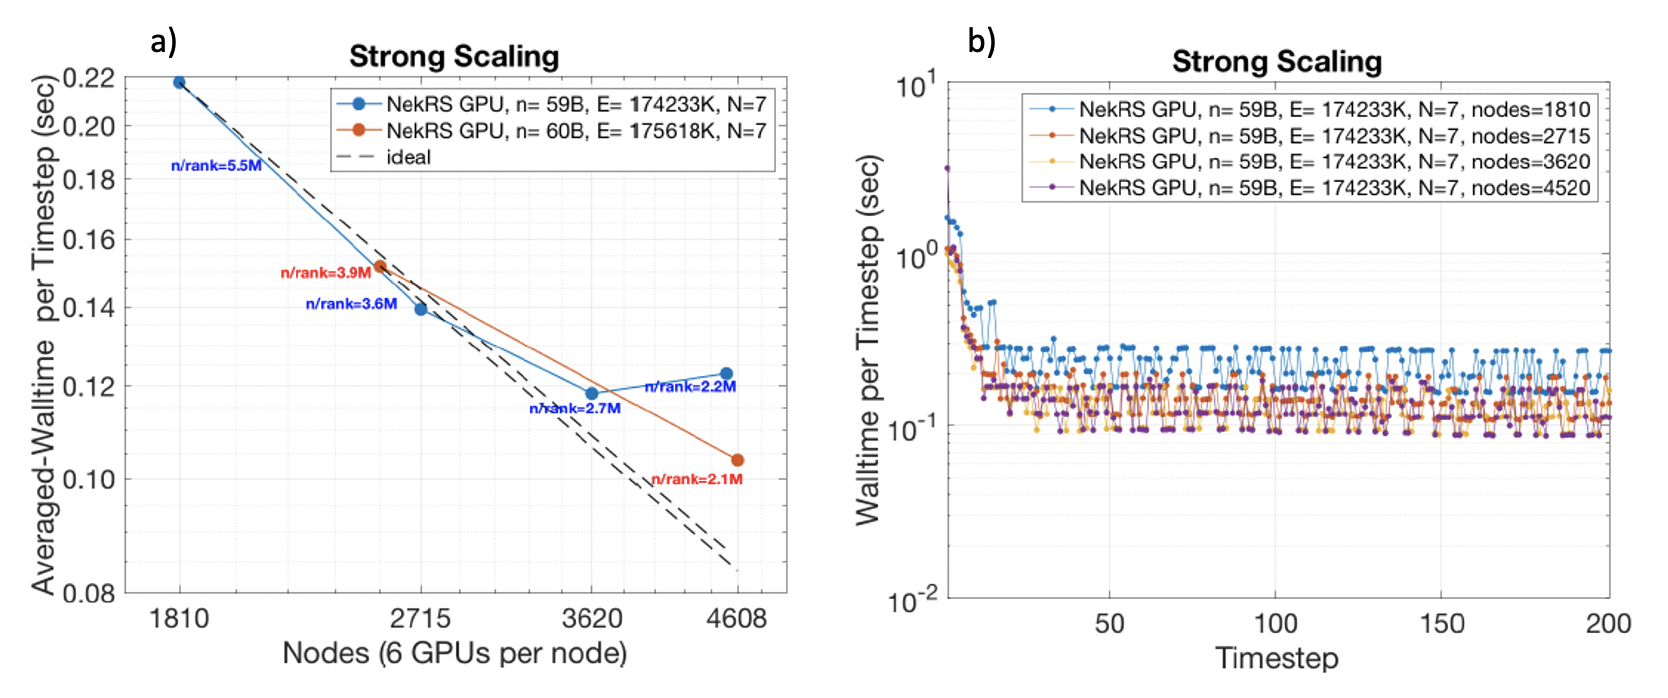
\includegraphics[width=0.99\textwidth]{./figures/full_core_strong.png}
\caption{Full core strong scaling study. a) average wall time per step. b) time per time step as simulation progresses. }
\label{fig:strong}
\end{figure}

The data collected has been used to generated updated FOM measurements in Table~\ref{tab:FOM}. This table includes both the measured FOM and the projected FOM to full machine for each of the cases. The cases with lower number of nodes should be considered a more accurate representation of full core projections for larger cases. The higher node counts are clearly below the strong scaling limit and likely do not have a sufficient number of elements and dofs per GPU.

We note that the FOM measured is significantly higher than the previous projected measurement on Summit: $1.44 \cdot 10^{11}$ dofs/s. The value reported show a 4.9x increase in projected values. We also note that the performance now is orders of magnitude higher than the FOM measured on Titan in 2018.

% Full core: n= 5.9762e+10 = E*N^3,          Previous 30M:  before (dofs/s)= 1.44506e+11
% node  rank   E                E/gpu  N  nstep  dt           cfl       t_step     avg_t_step       n/t_step     n/avg_t_step          1.44506e+11/(n/t_step)     1.44506e+11/(n/avg_t_step)
%4525  27150  174233000  6417   7  100    3.0e-04  0.58    9.34e-02   1.22e-01      6.3985e+11   4.8985e+11           4.4278e+00                      3.3898e+00
%4608  27648  174233000  6301   7  100    3.0e-04  0.58    9.01e-02   1.21e-01      6.6328e+11   4.9390e+11

 \begin{table} \centering \small
  % \resizebox{0.48\textwidth}{!}{
   \begin{tabular}{cccccc} \hline \hline
    Nodes & $E$/GPU & Fraction of machine & Average Time per step [s] & FOM (dofs/s) & Projected FOM (dofs/s) \\ \hline
    1810 & 	16043 & 0.393 &	0.2175  & $2.75 \cdot 10^{11}$ & $7.00 \cdot 10^{11}$ \\
    2715 &	10695 & 0.589 &	0.1395  & $4.29 \cdot 10^{11}$ & $7.28 \cdot 10^{11}$ \\
    3620 &	8021 & 0.786 &	0.1182  & $5.06 \cdot 10^{11}$ & $6.44 \cdot 10^{11}$ \\
    4525 &	6417 & 0.981 &	0.1229  & $4.87 \cdot 10^{11}$ & $4.95 \cdot 10^{11}$ \\
    4608 &	6301 & 1.000 &	0.121   & $4.94 \cdot 10^{11}$ & $4.94 \cdot 10^{11}$ \\
     \hline \hline
  \end{tabular}
   \caption{FOM measurement based on full core mesh. $E=174233000$, $N=7$.}
   \label{tab:FOM}
  \end{table}

\subsection{RANS full core simulations}
\label{sec:results2}

Several RANS simulations with the $k-\tau$ model have been performed as part of this campaign (see Table~\ref{tab:full core}). The numerical setup for the all the runs is consistent with the simulations discussed in Section~\ref{sec:nrs1}, which featured a verification study against Nek5000. In particular, crucial is the setup of the inlet boundary conditions. The cases have been run for a range of Reynolds numbers ($Re=10,000$ to $Re=60,0000$). The mesh was in fact  designed to support RANS simulations with $y+<1.0$ up to $Re=60,0000$.

Results from the periodic case (Case II) and the full height ($H=200.0 cm$) core case (Case III) yield identical results, at sufficient distance from the inlet. Sample results are provided in Figure~\ref{fig:vz} and Figure~\ref{fig:tke}. They illustrate a full core view and a detail for both the stream-wise velocity and the turbulent kinetic energy.  Both results are consistent with expectations and demonstrate inhomogeneous behavior near the thimbles and the boundaries of the core.

\begin{figure}[!ht]
\centering
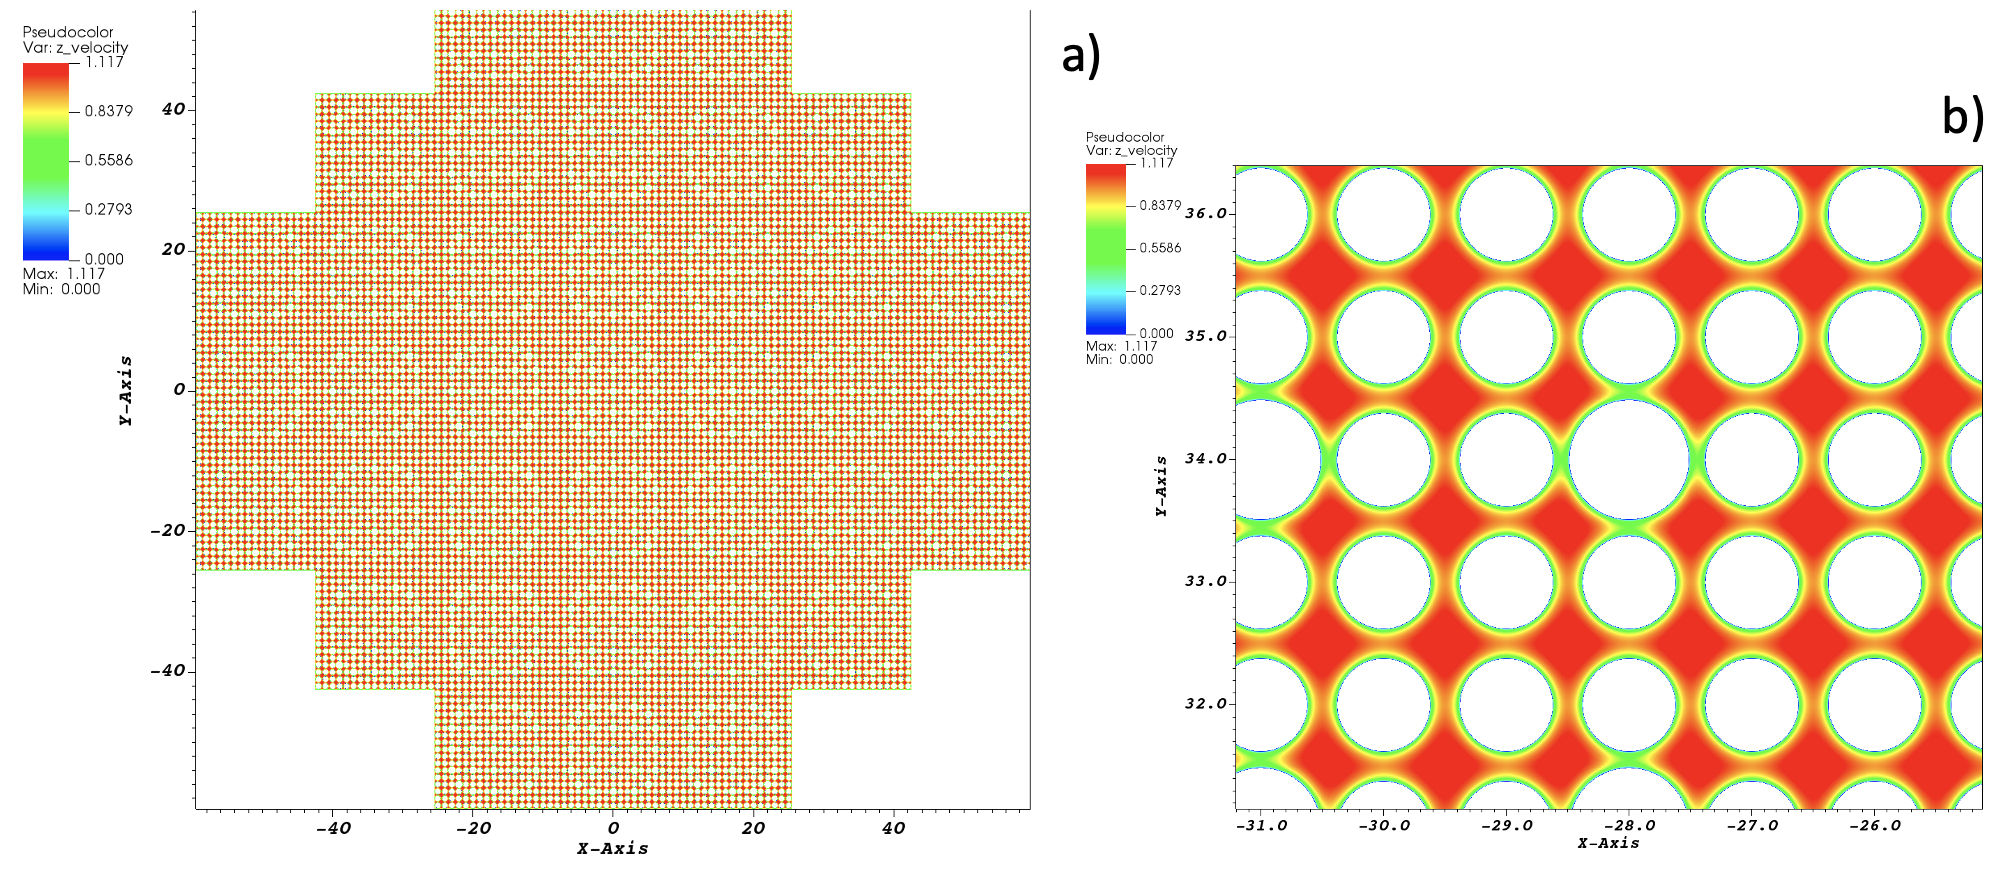
\includegraphics[width=0.99\textwidth]{./figures/periodic_vz.png}
\caption{Streamwise cross section of the velocity field ($Re=20,000$) in the fully developed region. Color plot of the streamwise velocity normalized by the bulk velocity. a) full core view. b) detail.}
\label{fig:vz}
\end{figure}

\begin{figure}[!ht]
\centering
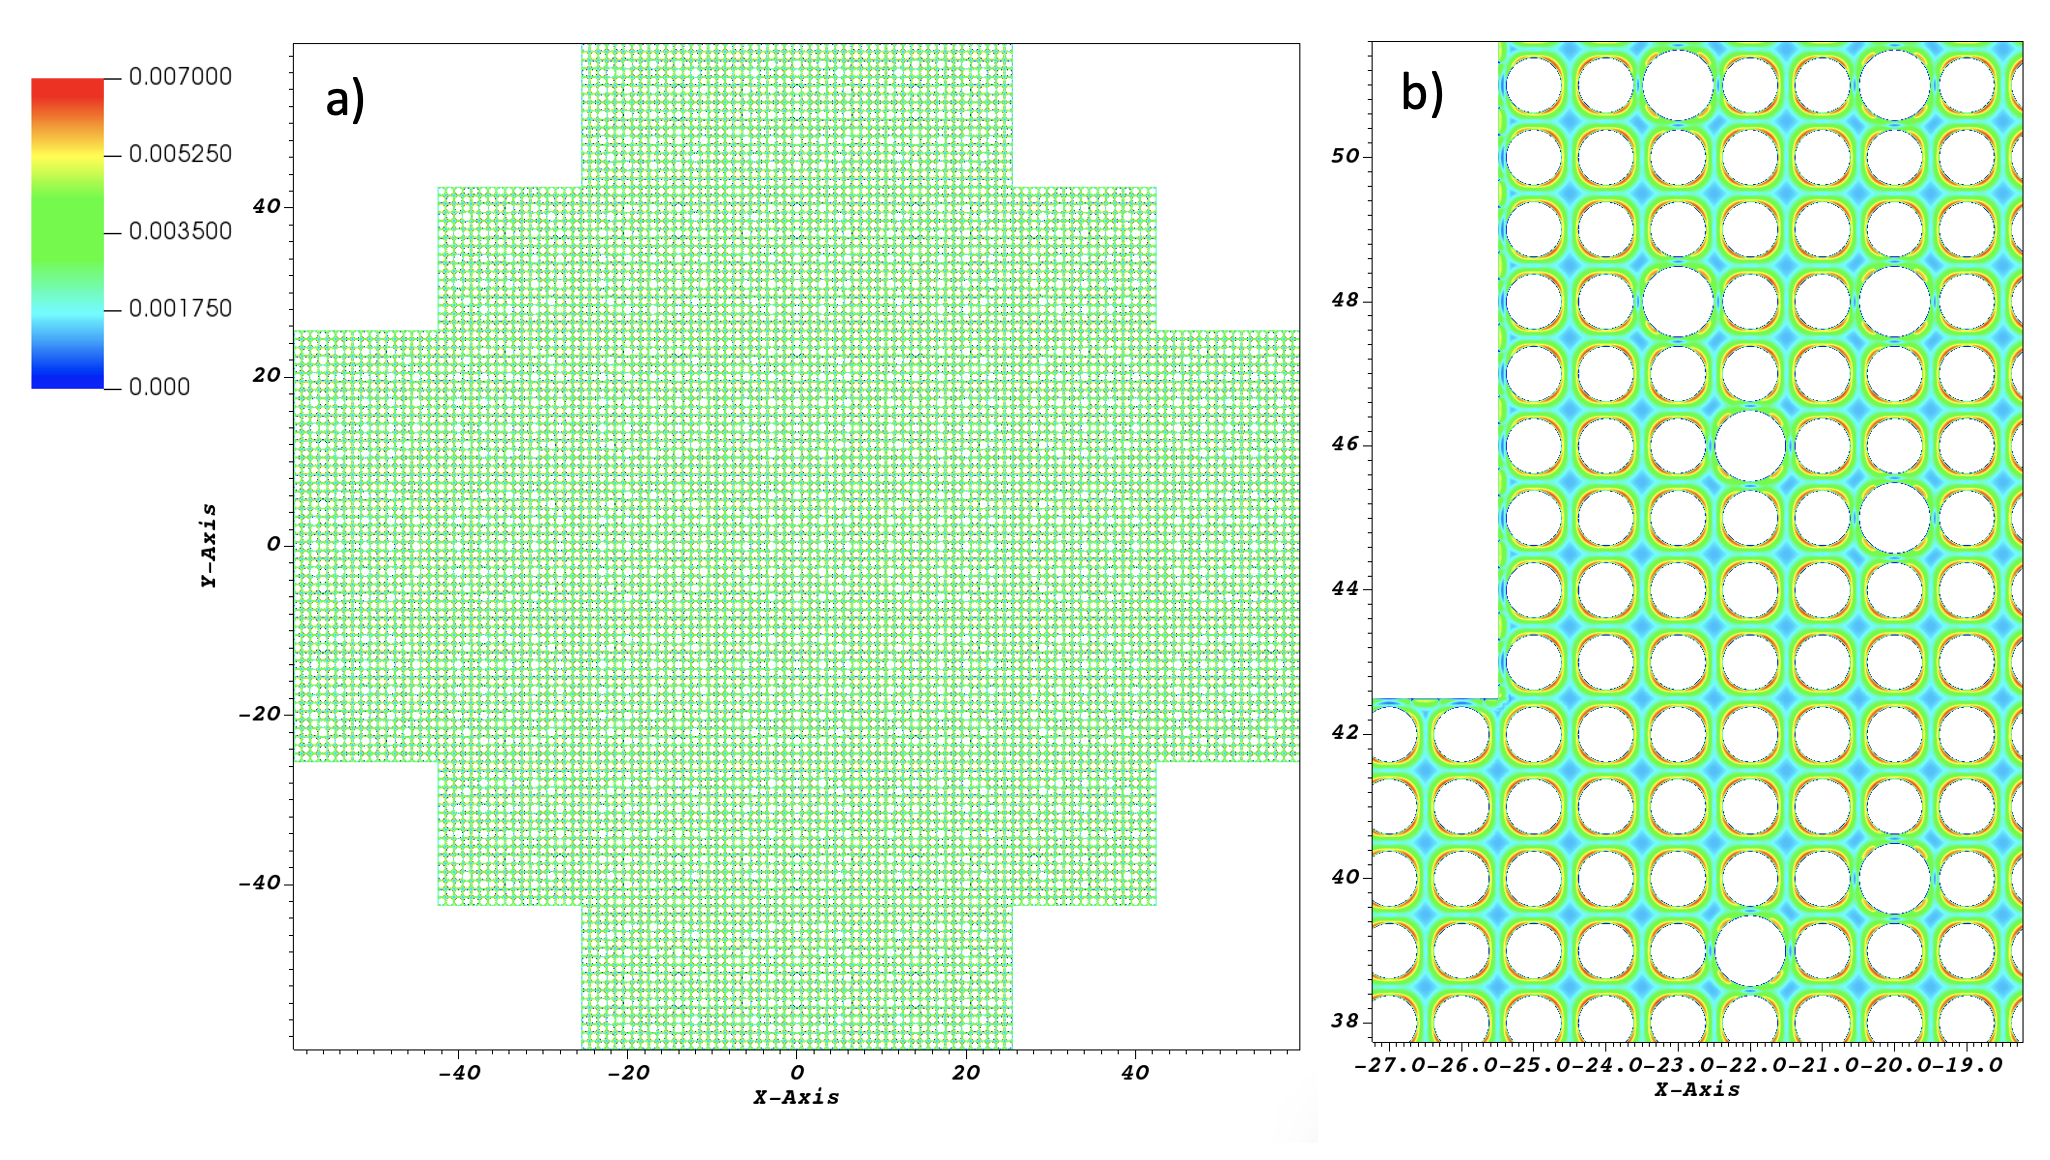
\includegraphics[width=0.99\textwidth]{./figures/periodic_tke.png}
\caption{Streamwise cross section of the velocity field ($Re=20,000$) in the fully developed region. Color plot of the turbulent kinetic energy. a) full core view. b) detail. }
\label{fig:tke}
\end{figure}

\subsection{RANS full core simulations with momentum sources}
\label{sec:results3}

The next step from Section~\ref{sec:results2} is to add appropriate momentum sources as developed through the procedure discussed in Section~\ref{sec:msm}. This was accomplished in cases IV and V.

 The momentum source was implemented in NekRS using the same approach developed in Nek5000 as leveraging as much as possible the same routines. In addition when extending to the full core, an appropriate interface was built to map the forces to the correct locations in the core based on a single assembly layout. An example of the layout of the forces is shown on a cross section in Figure~\ref{fig:msm}:
\begin{itemize}
    \item We assume every assembly has the same pattern;
    \item We choose to not place any force on the edge channels of each assembly;
    \item We simply repeat a simple 2x2 pattern in the interior of the assembly;
    \item We leave identical forces around the thimble, or none at all;
    \item We assume 5 grids axially.
\end{itemize}
We note that there is no particular restriction here and the choices were arbitrary to simplify the problem. The methodology allows to customize the forces as needed and have different patterns in different assemblies and at different heights.

We now show was sample results of the flow field in the full core. We pay particular attention to the cross flows. Figure~\ref{fig:msm1} shows the cross flows directly past the first grid span. The momentum sources induce significant cross flow in the core, consistent with 2x2 simulations performed. The values reached by the cross flows in both directions represent a high percentage of the bulk and are very important for heat transfer and mixing.

\begin{figure}[!ht]
\centering
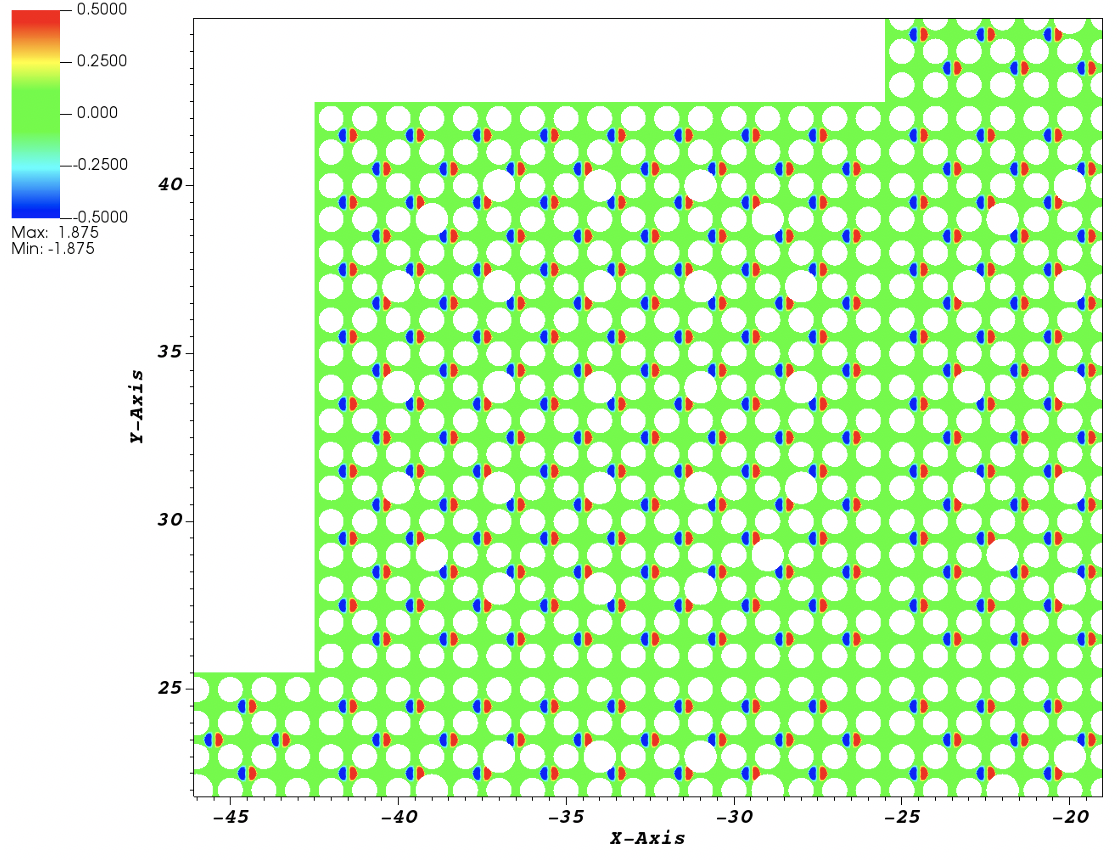
\includegraphics[width=0.99\textwidth]{./figures/1span_msm.png}
\caption{Detail of forces in full core simulation. Force in direction $y$. }
\label{fig:msm}
\end{figure}

\begin{figure}[!ht]
\centering
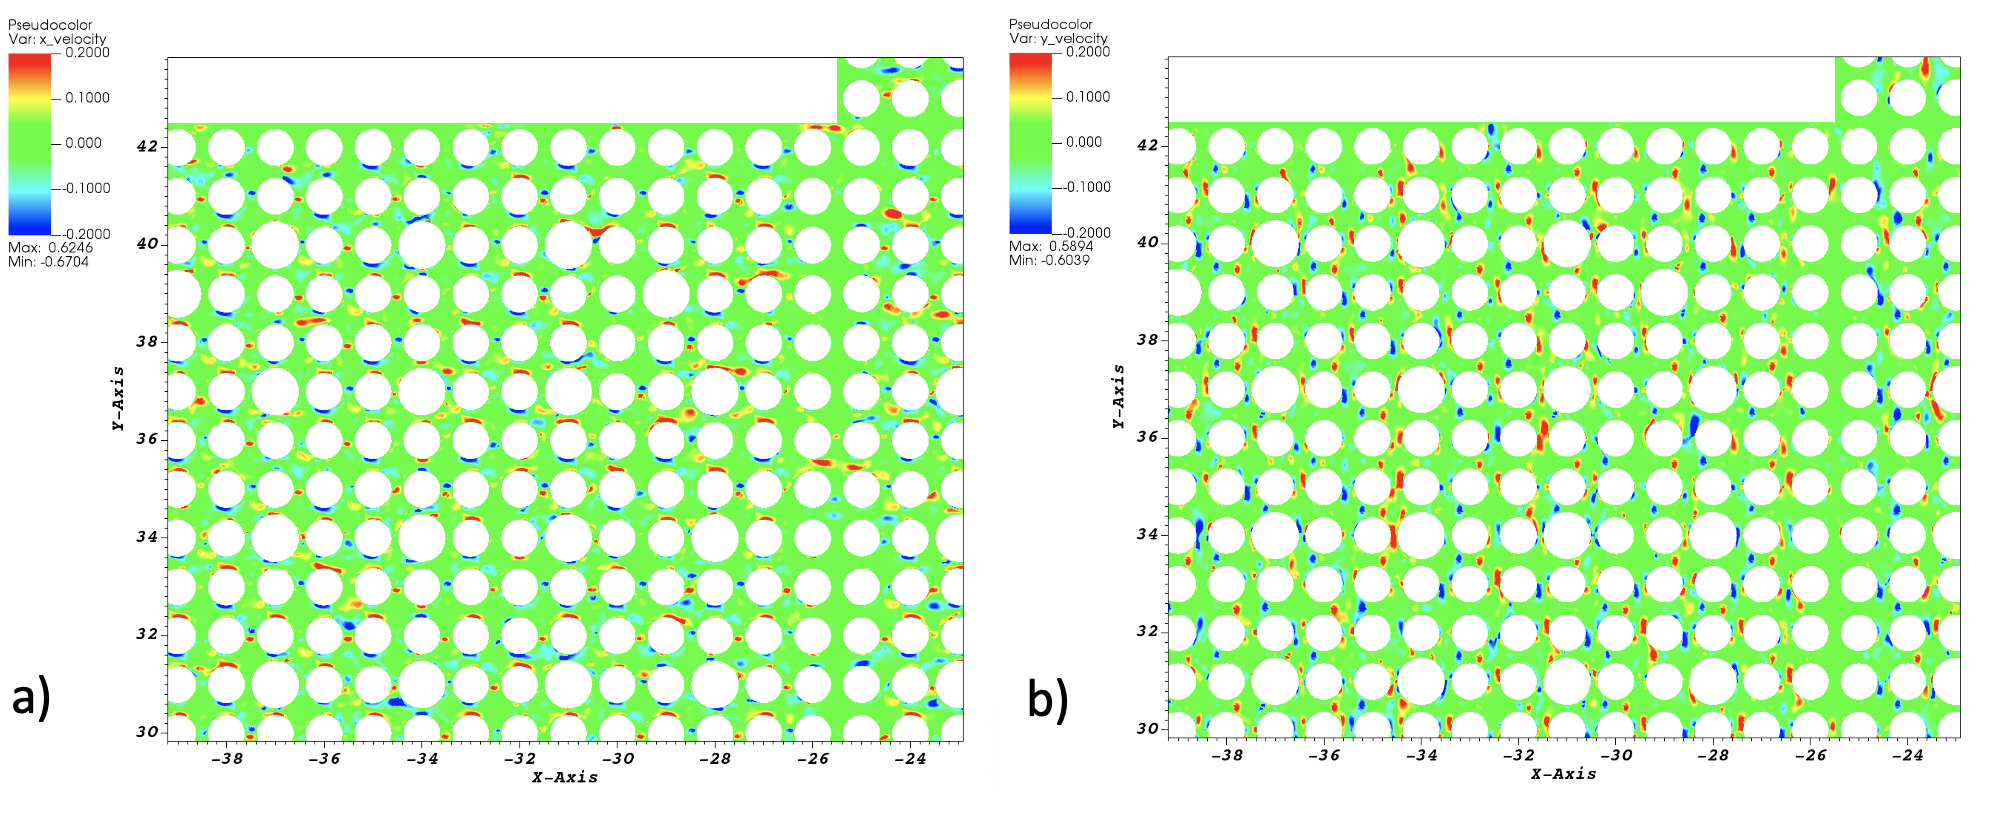
\includegraphics[width=0.99\textwidth]{./figures/1span_msm_v1.png}
\caption{Details of cross flow in full core after the spacer grid. a) Velocity in direction $x$. b) Velocity in direction $y$. }
\label{fig:msm1}
\end{figure}

\subsection{Conjugate heat transfer}
\label{sec:results4}

In addition to the full core cases demonstrated above, a quarter-height case (Case VI) was also performed for demonstration purposes of a conjugate heat transfer model representing each pin in the core. The mesh is consistent with previous 17x17 assembly calculations performed for coupled analysis with ENRICO. The gap and cladding are modeled explicitly as well as the fuel. A very preliminary result is shown in Figure~\ref{fig:cht}, for the beginning of transient.

\begin{figure}[!ht]
\centering
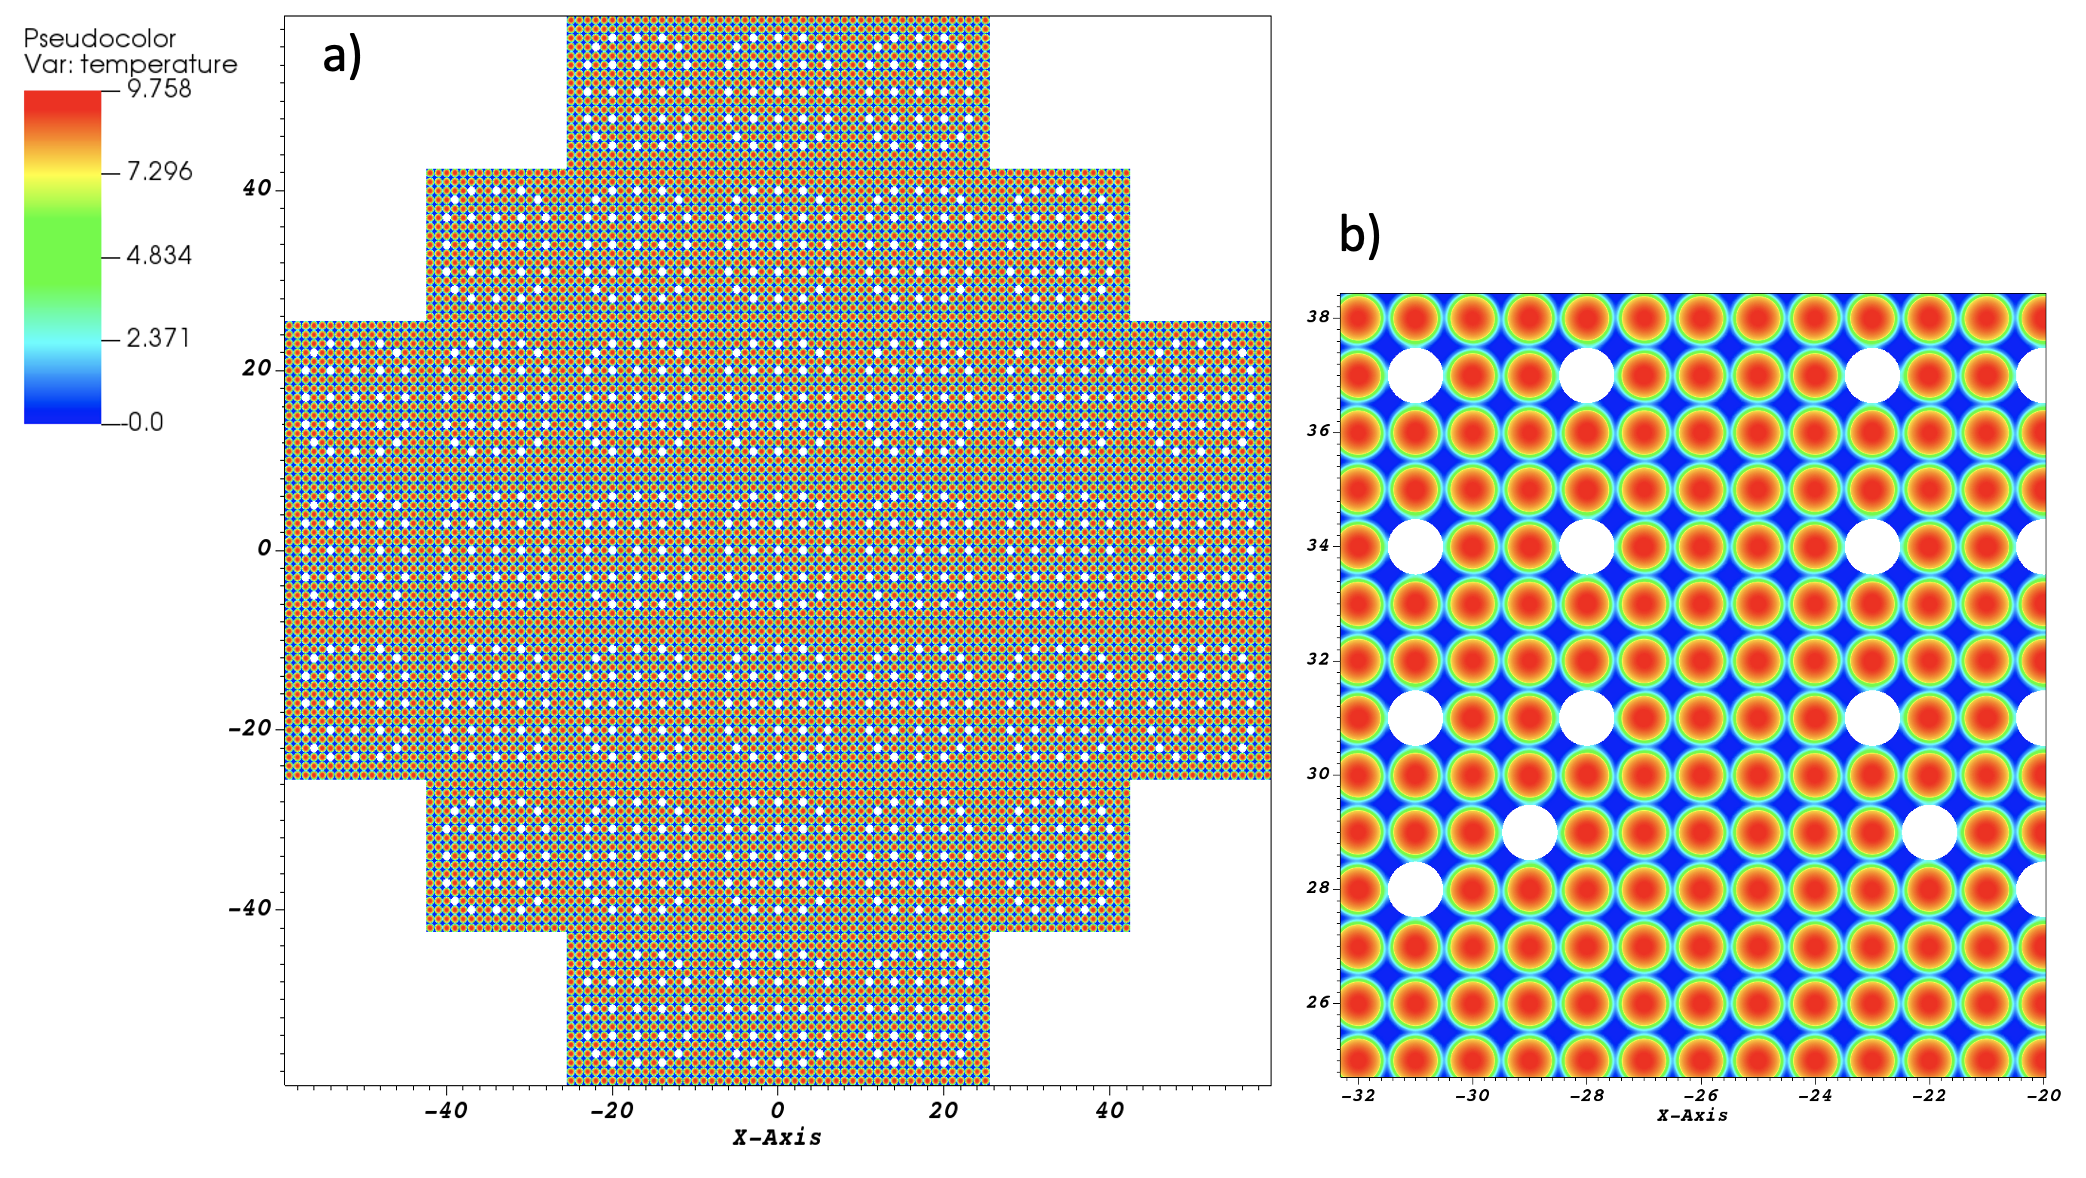
\includegraphics[width=0.99\textwidth]{./figures/quarter_cht.png}
\caption{Conjugate heat transfer results for full core, full view and detail. Temperature in arbitrary units.}
\label{fig:cht}
\end{figure}
